\part{Teoretická část}

\chapter{Historie XR}

\section{Počátky XR}

První pokusy o rozšířenou realitu pochází už z 50. let 20. století, kdy Morton Hellig, americký kinematograf, přivádí na svět své zařízení zvané Sensorama. Nejednalo se ovšem o headset, které si vybavíme dnes -- Sensorama bylo stacionární zařízení, vzhledově připomínající automat. Hellig toto zařízení nazýval "zážitkovým divadlem", které bylo schopné zobrazit 3D obraz, pouštět stereo zvuk a vytvářet vítr. Tím se od dnešní XR technologie zásadně liší; nepřijímá vstup uživatele. Sensorama se ovšem nedočkala úspěchu a známe ji jen jako historicky první pokus o virtuální realitu. \cite{otechnice}

Dalším průkopníkem rozšířené reality je Ivan Sutherland, americký vědec, který je často označován jako otec počítačové grafiky. Ve svém díle The Ultimate display (ultimátní displej) popsal virtuální realitu tak, jak ji známe dnes. Virtuální realitu si představoval jako helmu, do které odesílá obraz počítač v reálném čase. Uživatel se tak měl ocitnout ve fiktivním světě nerozpoznatelným od světa reálného. \cite{otechnice} \cite{ivan_sutherland_bio}

Tuto představu se Sutherland snažil realizovat se svými studenty. Společně vynalezli vůbec první headset pro virtuální realitu, zvané The Sword of Damocles -- tedy Damoklův meč. Vzhledem k jeho primitivnosti zobrazovalo pouze čtvercové místnosti tvořené z čar, které software následně transofrmoval do správné perspektivy. Pohyby sledovalo pomocí mechanického ramene připevněného ke stropu, ze kterého byl headset zavěšený. \cite{otechnice} \cite{Rheingold_1992}

\section{XR v armádě}

V 80. letech 20. století o XR projevila zájem armáda USA, ve snaze snadněji a efektivněji připravit americké piloty na ovládání letadel. Začala využívat speciálních simulačních kabin, které obsahovaly mimo jiné i speciální headset. Tento headset pomocí stereoskopického zobrazení informoval o průběhu letu, zobrazoval 3D mapy a snímky z radaru. Díky možnosti systém ovládat pomocí hlasu nebo pohybu očí se tento headset přibližuje k dnešnímu stavu VR, jelikož reaguje na vstup uživatele. \cite{otechnice}


\begin{figure}[H]
    \centering

    \begin{minipage}{.5\textwidth}
        \centering
        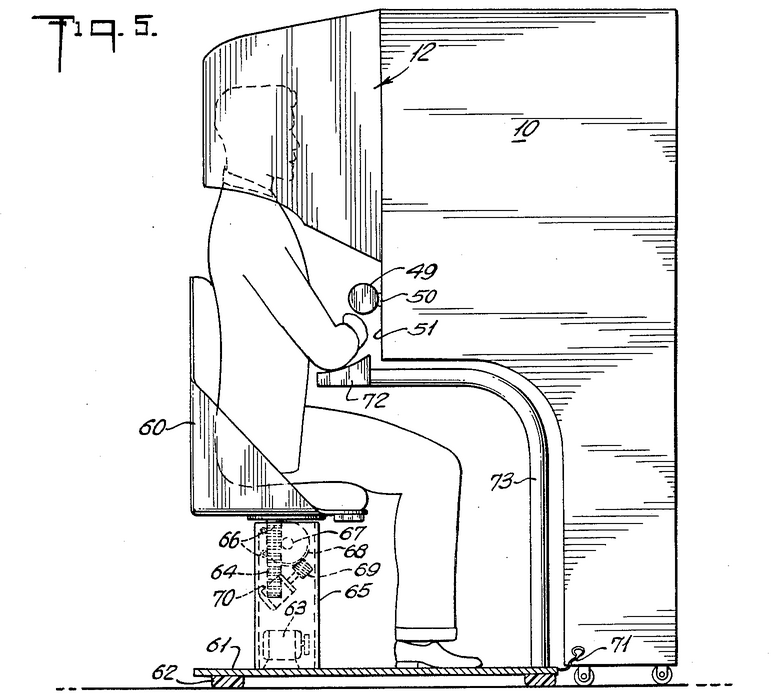
\includegraphics[height=120pt]{sensorama.png}
        \caption{Sensorama \cite{sensorama_patent}}
        \label{sensorama_fig}
    \end{minipage}%
    \begin{minipage}{.5\textwidth}
        \centering
        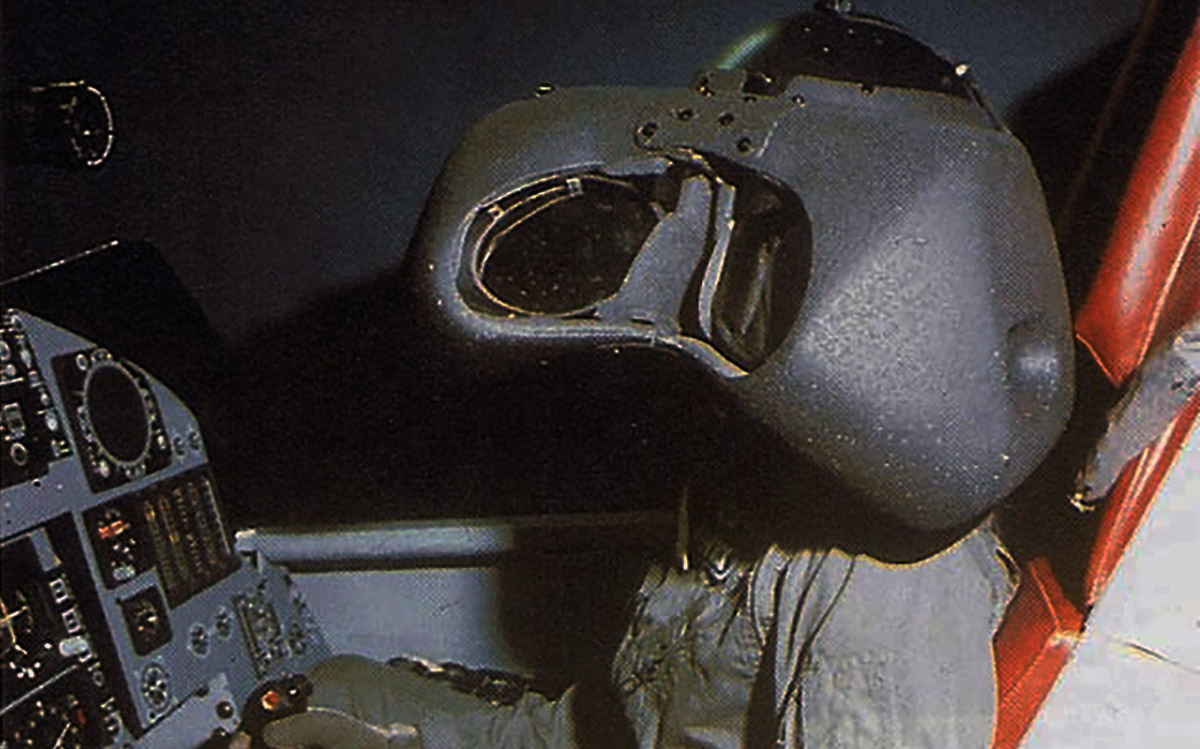
\includegraphics[height=120pt]{super_cockpit_helmet.jpg}
        \caption{Helma "Darth Vader", jedna z částí simulačního kokpitu \cite{super_cockpit_image}}
        \label{sensorama}
    \end{minipage}

\end{figure}

\section{Komerční dostupnost}

O počátku dostupnosti XR zařízení můžeme mluvit v 90. letech 20. století, kdy se tato technologie mohla dostat i do rukou obyčejných lidí. Dvojice zaměstnanců herní společnosti Atari, Jaron Lanier a Thomas Zimmermann, společně založili společnost VPL Research a začali s vývojem produktů pro XR. Zaměřili se na výrobu speciálních obleků a rukavic, které dokázaly přenést pohyby uživatele do počítače. Snímání pohybu ale nebylo dostatečně kvalitní a úspěch nezaznamenalo; dodnes je ovšem známé jako první cenově-dostupný XR systém. \cite{otechnice_2}

Herní společnosti na sebe také nenechaly dlouho čekat a začaly s vývojem VR konzolí pro hraní her. První takovou byla britská společnost Virtuality, která v roce 1991 uvedla na trh stejnojmenné zařízení představující arkádový stroj se stereoskopickými brýlemi. Kvůli vysoké pořizovací ceně nebylo dostupné pro domácnosti, Virtuality ovšem otevřela nespočet heren po celé Velké Británii. \cite{otechnice_2} \cite{independent_virtuality}

Do světa VR herních konzolí vstoupily i dnes známé japonské společnosti SEGA a Nintendo se svými SEGA VR a Virtual Boy. Obě tato zařízení však byla komerčními selháními. SEGA byla nucena kvůli technickým problémům vydání několikrát posunout a krátce po vydání skončila jeho výrobu. Nintendo sice své zařízení vydalo, ale rok po uvedení na trh jej stáhlo. Kvůli vysoké ceně a špatným grafickým schopnostem (konzole uměla zobrazit pouze červenou a černou barvu) si zálibu u hráčů nenašlo.\cite{otechnice_2}

\begin{figure}[H]
        \centering
        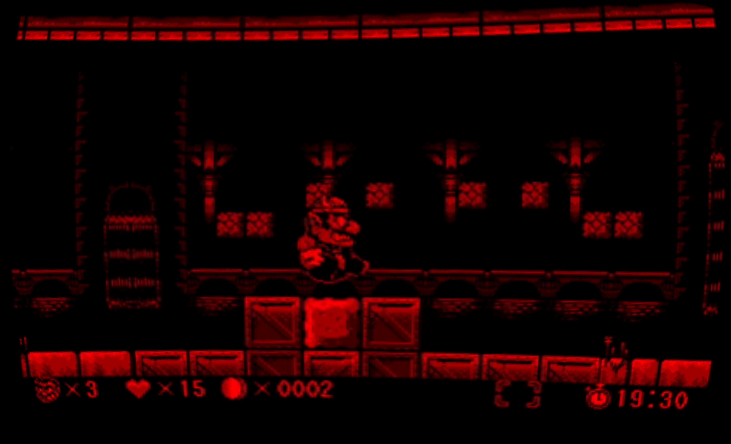
\includegraphics[height=120pt]{vboy.png}
        \caption{Červeno-černé zobrazení zařízení Virtual Boy \cite{vboy}}
        \label{vboy_red_display}
\end{figure}

\section{XR dnes}

Současná generace XR zařízení se začíná objevovat po roce 2010. Velkým průkopníkem v oblasti virtuální reality byla americká společnost Oculus, která oznámila zájem o vytvoření moderního VR systému. Jejich kickstarter\footnote{Webová stránka, kde začínající společnosti můžou žádat o finanční podporu veřejnosti. V Česku je známou alternativou \em Startovač.} se ukázal jako úspěch a přilákal pozornost jiných společností, zejména tehdejšího Facebooku (dnes Meta). Ten společnost Oculus odkoupil ještě před tím, než stačila vydat své první zařízení. Na to si zájemci museli počkat až do roku 2016, kdy bylo vydáno první zařízení zvané Oculus Rift CV1. Jeho konkurencí byl headset HTC Vive od tajwanské společnosti HTC. Tato zařízení fungovala pouze při propojení s počítačem; nebyla tedy samostatná. \cite{otechnice_3}

Vývoj mobilního VR (tedy takobho headsetu, který nepotřebuje počítač pro vykreslování obsahu) společnost Oculus konala za podpory korejského Samsungu, se kterým na trh uvedla Gear VR -- headset, který pro vykreslování používal mobilní telefon. Na podobném principu fungoval i experiment od Googlu zvaný Cardboard VR. Ten pro virtuální realitu používal pouze mobilní telefon a headset složený z kartonu (odtud název). Mobilní VR se v této době neuchytilo, zažilo ovšem velký rozmach v letech 2019-2020 po vydání headsetu Oculus Quest (dnes Meta Quest), který byl plně samostatný a používal upravenou verzi OS Android. Hry pro tento headset jsou upravené, aby běžely na Androidu, nicméně existuje možnost jej připojit k počítači a hrát hry pro "nesamostatné" headsety. \cite{otechnice_3}

Díky technologickým pokrokům a zmenšování hardwaru se také začala objevovat zařízení pro smíšenou realitu, která pomocí snímačů a pohledu z kamery umožnila vkládat virtuální předměty do reálného světa. Forem měla mnoho; například upravené optické brýle s malým displejem nebo speciální headsety. O tato zařízení se pokoušeli technologičtí giganti jako Google a Microsoft. Kvůli vysokým pořizovacím cenám ale tato zařížení u jednotlivců neuspěla a tyto společnosti s nimi dodnes cílí na pracovní prostředí. \cite{google_glass_mobilenet}

Velmi dostupné byly naopak aplikace používající augmentovanou realitu. AR byla integrována do již existujících zařízení, především jako technická dema. Běžnou metodou sledování pohybu bylo, pro svou nenáročnost, sledování speciálních předmětů či kartiček, které zařízení rozpoznalo, určilo jejich otočení a naklonění a následně zobrazilo obsah. Zlom nastal, když Google vydal ARCore, \gls{SDK} pro AR, který umožnil vývojářům sledovat pohyb mobilního telefonu pouze pomocí pohledu z kamery. Vývojáři se tím pádem mohli zaměřit pouze na vývoj jejich aplikací a her, protože nemuseli investovat čas a peníze do technologie sledování pohybu. Právě v této době vznikla většina aplikací a her, které známe. Za zmínku stojí například Pokémon GO. \cite{enwiki:1182789097}

\chapter{Hardware}
lorem ipsum

něco o trackování, výrobcích, atd. zmínit trackovací systém bez věží od Meta/FB

rozlišit 6dof vs 3dof

\chapter{Software}
lorem ipsum

zmínit OpenXR, WebXR jakožto API co pohánějí XR

rozlišit PCVR na windows a mobilní VR na bázi androidu